\Chapter{Introduction}
%%%%%%%%%%%%%%%%%%%%%%%%%%%%%%%%%%%%%%%%%%%%%%%%%%%%%%%%%%%%%%%%%%%%%%%%%%%%%%%%%%%%%%%%%%%%
%%%%%%%%%%%%%%%%%%%%%%%%%%%%%%%%%%%%%%%%%%%%%%%%%%%%%%%%%%%%%%%%%%%%%%%%%%%%%%%%%%%%%%%%%%%%
\Section{Motivation} \label{sec:motivation}
%%%%%%%%%%%%%%%%%%%%%%%%%%%%%%%%%%%%%%%%%%%%%%%%%%%%%%%%%%%%%%%%%%%%%%%%%%%%%%%%%%%%%%%%%%%%
%%%%%%%%%%%%%%%%%%%%%%%%%%%%%%%%%%%%%%%%%%%%%%%%%%%%%%%%%%%%%%%%%%%%%%%%%%%%%%%%%%%%%%%%%%%%

A new generation of accelerators dedicated to High-Energy Physics
(HEP) would likely be of the TeV scale. Reduction in the size and cost
of such machines is key to their feasibility. 
Technologies for high gradient acceleration for future HEP machines is an area of active research.
Traditional accelerating gradients are on the order of 10's of MV/m
with the power source being a klystron gallery.
High gradient structures and schemes such as the 
short pulse, two-beam acceleration (TBA) scheme 
at the Argonne Wakefield Accelerator (AWA) facility
use novel structures to reach 100's of MV/m or more. 
A goal of the AWA group is to demonstrate fully staged TBA, 
achieving a gradient of 250 MV/m. If successful, this would
be the only facility in the world capable of such gradients used for
acceleration of a beam.

TBA requires a drive beam to pass through a decelerating structure and
lose energy through wakefield generation. The electromagnetic wake
is coupled from the decelerator into an accelerating structure, where
the electric field is used to accelerate a second beam. 
This requires two complete and separate beamlines 
operating synchronously with each other.  
The wakefield structures can be metallic or dielectric on either beam line. 
Dielectric structures, having no irises, are simple to manufacture and have demonstrated
high gradient capability at \SI{100}{MV/m} \cite{WeiPaper}. 

The Compact Linear Collider (CLIC) collaboration proposes a similar TBA scheme with
a \SI{240}{ns} pulse length. This limits the acceleration gradient
to roughly \SI{150}{MV/m} at room temperature due to rf breakdown \cite{CLICdesignReport}.
Higher gradients could be reached when driven by a very short drive
beam pulse, such as the \SI{20}{ns} pulse length proposed by AWA \cite{WeiPaper}. 
While the peak power and gradients are considerably larger in the short pulse scheme, 
the average power is still feasible and within current technology capabilities.
While the two groups vary on approach, they agree that TBA would 
require less infrastructure when constructing a linear TeV scale machine, 
versus the cost of more conventional technology. 

A case study was done comparing the infrastructure 
needed using traditional \SI{50}{MW} klystron sources versus the TBA case.
It would take roughly 35,000 klystrons to construct a linear machine to deliver the same 
\nrnote{add explanation here YT}
\SI{9.2}{TW} power required in the CLIC design specification reports \cite{CLICdesignReport}. 
With TBA, CLIC projected a \SI{3}{TeV} energy at a length of \SI{48}{km}.
In contrast, the Next Linear Collider (NLC) collaboration projected a \SI{1}{TeV} machine 
with length \SI{26}{km}, using X-band klystrons \cite{NLC}. 
This drastic difference occurs in the infrastructure needed to generate and transfer
RF power in the two cases. In TBA, a high charge bunch train is generated in 
a photoinjector and propagated downstream using conventional technology 
(accelerating structures, quads, dipoles, etc). After reaching the design energy,
the bunch train
is focused into specially designed wakefield structures (decelerating structure).
RF power is extracted in the decelerating structure and supplied to the witness 
beam line through a waveguide connection. This has two benefits over traditional klystron technology.
One, you can have structures at higher frequencies (any multiple of the machine frequency), 
which helps push the gradient. Readily available and production klystrons are limited in this aspect.
Second, all the waveguide infrastructure needed to connect a klystron to the accelerating 
structures is eliminated. There is an initial cost near the photoinjector 
and for waveguide between the drive and witness lines, 
but downstream much of the infrastructure costs are eliminated.
Theoretically, TBA can deliver the same amount of power as conventional methods with less 
infrastructure, and therefore lower cost, in the case of a large machine. 

Before a detailed understanding of the power and infrastructure trade-offs 
can be obtained, the feasibility of staged TBA must be demonstrated.
Demonstration of staging is especially important, 
as no high-energy machine can be built without staging.
Staging is the ability to use two successive accelerating modules to synchronously accelerate 
the same particle bunch. While simple in principle, the difficulties 
in achieving staging should not be underestimated. 
Demonstration of staging proves that a TBA scheme can be scaled to high energies, and whether it is 
feasible to use such methods. Single stage TBA, and staging 
in a simplified scheme have been demonstrated at the AWA in 2016 \cite{tba2017}.
In the simplified scheme, both bunch trains travel through two decelerating stages.
This causes energy loss in stage 1 as the the second bunch train travels to stage 2.
\begin{figure}
	\begin{center}
		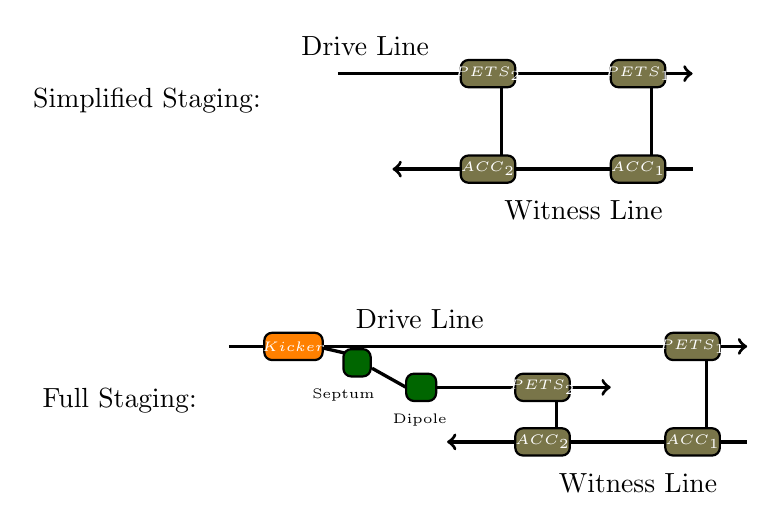
\begin{tikzpicture}[scale=\textwidth/35cm, text=black]
		\def \gunleft {-1.0}
\def \gunright {0.3}
\def \loneright {1.0}
\def \ltworight {2.0}
\def \lthreeright {3.0}
\def \lfourright {4.0}
\def \lfiveright {5.0}
\def \lsixright {6.0}
\def \quadone {7.3}
\def \quadfour{16}

%Full Staging
\draw[very thick, ->] (8,1) -- (27,1);

%Line between kicker and septum
\node[] at (15,2) {Drive Line};
\node[] at (23,-4) {Witness Line};
\draw[very thick] (\lsixright+5.2,1.0) -- (12.5,0.7);

%Kicker 
\draw[fill=orange,  thick, rounded corners =0.1cm] (\lsixright+3.3,0.5)rectangle ({\lsixright+0.84+4.6},1.5) node[pos=.5, white] {\tiny $Kicker$};
%Septum
\node[] at (12.2,-0.8) {\tiny Septum};
\draw[fill=black!60!green,  thick, rounded corners =0.1cm] (12.2,0.9)rectangle ({13.2},-0.1) node[pos=.5, white] {};
%Line between kicker and septum
\draw[very thick] (13.25,0.2) -- (14.5,-0.5);
%Dipole
\node[] at (15,-1.7) {\tiny Dipole};
\draw[fill=black!60!green, thick, rounded corners =0.1cm] (14.5,0.0)rectangle ({15.6},-1.0) node[pos=.5, white] {};
%Line between dipole and quads
\draw[very thick, ->] (15.6,-0.5) -- (22,-0.5);
%Witness
\draw[very thick, <-] (16,-2.5) -- (27,-2.5);
%Waveguide
\draw[very thick] (20,-0.5) -- (20,-3);
%Waveguide
\draw[very thick] (25.5,1.5) -- (25.5,-3);
%PETS2
\draw[fill=black!60!yellow,  thick, rounded corners =0.1cm] (18.5,0.0)rectangle (20.5,-1) node[pos=.5, white] {\tiny$\text{PETS}_2$};
%PETS1
\draw[fill=black!60!yellow,  thick, rounded corners =0.1cm] (24,1.5)rectangle (26,0.5) node[pos=.5, white] {\tiny$\text{PETS}_1$};
%ACC2
\draw[fill=black!60!yellow,  thick, rounded corners =0.1cm] (18.5,-2)rectangle (20.5,-3) node[pos=.5, white] {\tiny$\text{ACC}_2$};
%ACC1
\draw[fill=black!60!yellow,  thick, rounded corners =0.1cm] (24,-2)rectangle (26,-3) node[pos=.5, white] {\tiny$\text{ACC}_1$};



%Simplified Staging



\draw[very thick, ->] (12,11) -- (25,11);

%Line between kicker and septum
\node[] at (13,12) {Drive Line};
\node[] at (21,6) {Witness Line};

%Witness
\draw[very thick, <-] (14,10-2.5) -- (25,10-2.5);
%Waveguide
\draw[very thick] (18,11.5) -- (18,7);
%Waveguide
\draw[very thick] (23.5,11.5) -- (23.5,10-3);
%PETS2
\draw[fill=black!60!yellow,  thick, rounded corners =0.1cm] (16.5,11.5)rectangle (18.5,10.5) node[pos=.5, white] {\tiny$\text{PETS}_2$};
%PETS1
\draw[fill=black!60!yellow,  thick, rounded corners =0.1cm] (22,11.5)rectangle (24,10.5) node[pos=.5, white] {\tiny$\text{PETS}_1$};
%ACC2
\draw[fill=black!60!yellow,  thick, rounded corners =0.1cm] (16.5,8)rectangle (18.5,7) node[pos=.5, white] {\tiny$\text{ACC}_2$};
%ACC1
\draw[fill=black!60!yellow,  thick, rounded corners =0.1cm] (22,8)rectangle (24,7) node[pos=.5, white] {\tiny$\text{ACC}_1$};








		\node[fill=white, inner sep=2pt] (txt2) at (5,10) {Simplified Staging:};
		\node[fill=white, inner sep=2pt] (txt2) at (4,-1) {Full Staging:};
		\end{tikzpicture}
	\end{center}
	\caption{Simplified drawing of the two staging schemes.
		The arrows indicate what direction the beams travels.
		``Simplified staging'' refers to experiments that took place at the AWA  prior to 2017.
		``Full Staging'' refers to the TBA scheme that is the subject of this thesis.
		Installation efforts are currently ongoing.
		PETS stands for Power Extraction and Transfer Structure, and ACC stands for Accelerating structure. 
		The subscript on each structure refers to which stage the structures belong to (first or second). 
		In the simplified staging scheme the stages are not separated, meaning bunch train two travels
		through and loses energy in the first stage before reaching the second stage.
		This is prevented by separate beam lines in the full staging layout. }
	\label{fig:one}
\end{figure}

Fully staged TBA introduces a fast rise time kicker
and subsequent dogleg-like beam line. In this scenario, bunch trains can be 
directed to two independent decelerating structures. 
Therefore you can extract the maximum amount of power in each stage.
The thesis work included experimental preparation of fully staged TBA, 
along with beam line design and optimization. 


%%%%%%%%%%%%%%%%%%%%%%%%%%%%%%%%%%%%%%%%%%%%%%%%%%%%%%%%%%%%%%%%%%%%%%%%%%%%%%%%
\Section{Power Generation}

Wakefields are RF energy that is generated in a structure when a beam passes through it. 
The electromagnetic fields
associated with the beam induce surface charges on the structure walls.
If the material has a finite conductivity, discontinuities, or both, the
surface charges will lag behind the beam. These charges then induce
transverse and longitudinal field components in the structure as they
pass irregularities. The resulting electric potential
generated by the beam is commonly called the wake potential, which
is defined as the total voltage lost by a charge following the beam
at some finite distance \cite{SLACwakefields}. The wake potential is 
often calculated numerically using a simulation code. Once calculated, 
the wake potential can then be used to determine how much energy the 
beam will lose after passing through a specific structure. 

Metallic structures used in simplified staging experiments at the AWA, consist of 34 cells and irises. 
The dielectric PETS are also under development at the AWA. 
They consist of a cylindrical metal tube lined with a dielectric \cite{PETSeq}, 
see Fig. \ref{fig:PETS}. Both are candidates for use in full staging, and 
the dielectric structures are especially attractive due to their simplicity. 
The simple geometry reduces cost and complications during fabrication.
It is also easier to damp higher order modes. For example, longitudinal slots in the metal tube surrounding
the dielectric can disrupt the current that supports higher order modes.   
\begin{figure}
	\begin{center}
		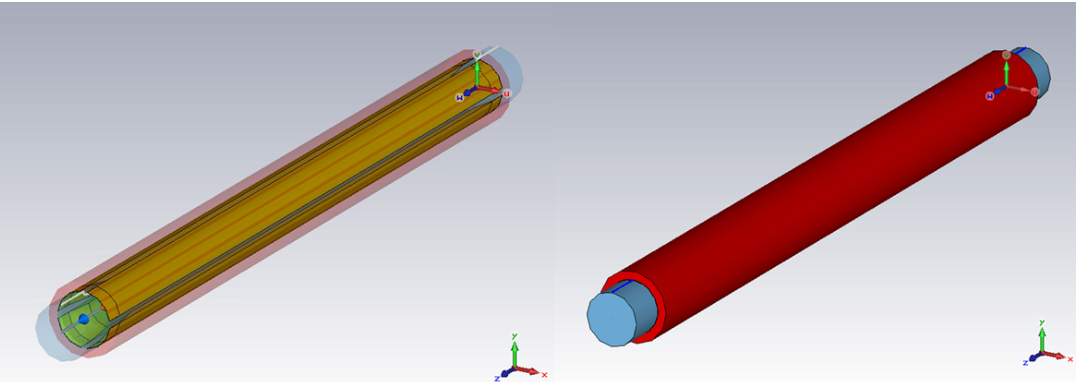
\includegraphics[width=0.8\textwidth]{images/pets-cst.png}
		\caption{CST drawing of a dielectric PETS design, courtesy C. Jing at AWA. 
		The structure is a dielectric tube with a metallic coating. Blue shading 
	indicates the vacuum aperture.}
		\label{fig:PETS}
	\end{center}
\end{figure}
In addition to simplicity in fabrication, an analytic solution for the electric fields
in a cylindrical dielectric is achievable using Maxwell's equations and theory developed
by Rosing and Gai \cite{RosingWei}: \nrnote{move general eq earlier - YT}
\begin{equation}
E^m_z\left(r,\theta,z_0\right)= \frac{N}{\sigma \sqrt{2\pi}}\int_{-\infty}^{z_0}E^m_z\left(r,\theta,z\right)e^{-\left[\frac{\left(z_0-z\right)^2}{2\sigma^2}\right]}\,\,dz , 
\end{equation}
where $r$, $\theta$, and $z$ define the cylindrical coordinate space, 
$z_0$ is the distance behind the drive bunch where the field is being calculated, 
$N$ is the number of particles in the bunch, and $\sigma$ is the bunch length.
This form of the electric field depends on the material properties of the structure
\nrnote{Add more equations here to show permittivity instead of refer to it? - YT}
(see the full expression for $E_z^m$ in \cite{RosingWei}, for the permittivity, $\epsilon$, dependence).
Materials with auspicious permittivities can be chosen to support larger fields
in the longitudinal direction, the field component 
used for acceleration.   
After maximizing the electric field, the wake potential, $W_z$, can be calculated: 
\begin{equation}
W_z\left(z\right)= -\frac{1}{Q} \int_{0}^{L} E_z \left(z,\frac{\left(z+z_0\right)}{c}\right)\,\,dz,
\label{eq:wakepotential}
\end{equation} 
where $c$ is the speed of light, $Q$ is the charge, 
and $L$ is the location where the charge leaves the cavity \cite{SLACwakefields}.
As shown by the negative sign in equation \ref{eq:wakepotential}, wakefields are a source of 
energy loss in the beam, often disrupting desired particle trajectories, 
and were considered an undesirable side effect.
However, people studying wakefields quickly realized that fields
generated by beams in certain structures resemble fields produced by external RF power 
applied to cavities or waveguides used to accelerate particle beams.
Hence, the idea arose to use wakefields as a power source for beam acceleration. 

Note, while wakefield generation is a crucial tool used in TBA at the AWA, the thesis does not include 
structure design. Other members of the AWA group have designed the PETS and accelerating
structures. The thesis will focus on beam line design and beam dynamics. 



\Subsection{Ideal power output from PETS}
The acceleration gradient achieved at the AWA will depend heavily 
on the PETS and accelerating structure designs, and beam quality 
provided to those structures. This section will focus on the 
structures in use at the AWA and the design specifications of future 
dielectric structures. All PETS and accelerating structures 
used in the simplified staging scheme were metallic. 
While the field is not as high as a dielectric structure would provide,
they have proven to be a great first step 
in determining whether or not TBA was possible at the AWA. Given 
the simplified scheme, predictions could be made for the acceleration 
gradient and energy gain, based on well-known principles. 

A few key equations demonstrate the relationship between beam 
parameters and the resulting power generated in the decelerating structures.  
Starting with the timing, each bunch is separated
in time by $T_{b}=$\SI{769}{ps}, and the average beam current can be written as $I=\frac{Q}{T_{b}}$, 
where $Q$ is the ideal bunch charge.
The bunches are finite and Gaussian in the longitudinal direction. Therefore the fields 
generated by the bunch are related to the shape, and do not fill the structure as an
rf pulse from a klystron would.  A form factor, $\Phi$, 
must be calculated to scale the resulting rf power accordingly. 
The form factor is calculated 
by taking the Fourier transform of the Gaussian charge distribution, $f(z)$\cite{PETSeq}: 
\begin{equation}
f\left(z\right) = \frac{q}{\sigma_z \sqrt{2\pi}}\;exp\left(-\frac{z^2}{2\sigma^2_z}\right),
\end{equation}   
\begin{equation}
\Phi = \left|\frac{1}{q}\int_{-\infty}^{+\infty}f\left(z\right)e^{-jk_z z}z\right|,
\end{equation}
\begin{equation}
\Phi=exp\left[\frac{-(k_{z}\sigma_{z})^{2}}{2}\right] \nonumber,
\end{equation}
where $k_{z}=\frac{2\pi}{\lambda_{z}}$ is the longitudinal wave number
of the decelerating structure, and $\sigma_{z}$ is the rms bunch length \cite{PETSeq}. 
Note the subscript z refers to the characteristics of the structure and bunch in the longitudinal
direction. 
As an example, Figure~\ref{fig:form} shows the expected form factor for full staging.
\begin{figure}
	\centering
	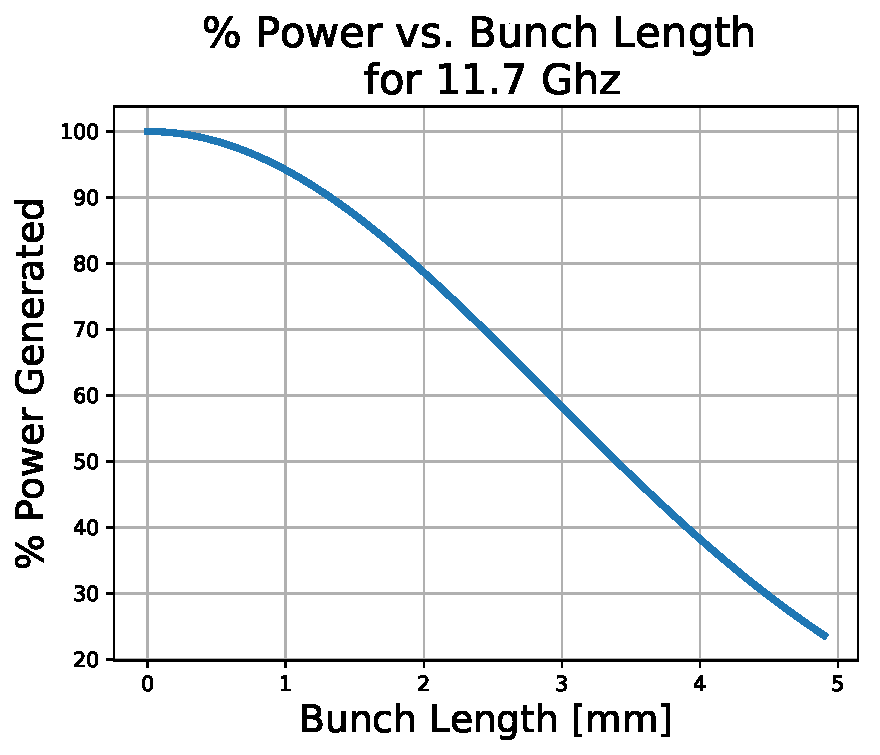
\includegraphics[width=0.75\textwidth]{images/formfactorsqrd}
	\caption{Form factor as a function of bunch length for full staging (\SI{40}{nC}).}
	\label{fig:form}
\end{figure}

When a Gaussian bunch, as described above, travels through a 
decelerating structure, it radiates an electromagnetic field and 
power is lost in the structure. Conservation of energy dictates 
that the amount of power left in the beam 
after it travels some distance through the structure is equal to 
the total power the beam started with
minus the power lost to the structure through electromagnetic radiation. 
Using this concept, Whittum derived an expression for the power, $P_t$, 
generated by the beam as it travels through a structure \cite{Whittum}: 
\begin{equation}
P_t = \frac{E^2_a}{2 \alpha R}\, ,
\label{eq:power1}
\end{equation} 
where $\alpha=\frac{\omega}{2Q_{d}v_{g}}$ is the attenuation constant of the 
decelerating structure \cite{CLICdesignReport, Whittum}, 
$v_g$ is the group velocity of the structure, $R$ is the shunt impedance
per unit length, and $E_a$ is the longitudinal electric field in the structure
generated by the beam. 
$E_a$ can be written with respect to 
the structure parameters and beam current \cite{PETSeq}. 
This equation quantifies how much power in the bunch is transferred into usable electric field.
The form factor, $\Phi$, can then be used to scale the electric field before 
solving for the power: 
\begin{equation}
E_a\left(L\right) = \frac{Iw}{2 v_g \alpha} \frac{R}{Q} \left(1-e^{-\alpha L}\right) \Phi.
\end{equation}
The electric field plugged into equation \ref{eq:power1} then gives the power provided
by the beam through wakefield generation,
\begin{equation}
P_{t}(t)=\frac{\omega\,I^{2}}{4\,v_{g}}\frac{R}{Q_d}\left(\frac{1-e^{-\alpha L}}{\alpha}\right)^2\Phi^{2},
\label{eq:power}
\end{equation}
where $I$ is the beam current as defined above, and $Q_{d}$ is the quality factor for the decelerating
structure. Note, the full derivation of equation \ref{eq:power} can be found in references
\cite{PETSeq}. The ratio of $\frac{R}{Q}$ is a parameter that quantifies the coupling between
the beam and the mode(s) in the structure \cite{Whittum}, as not all the the power stored in 
the beam is lost to the structure. Due to the complex geometry of metallic structures,
the value of $\frac{R}{Q}$ is often calculated in electromagnetic codes such
as CST Microwave Studio. 

\Subsection{Structure Parameters}
Both metallic and dielectric PETS have been tested at the AWA, 
and are candidates for the fully staged beam line. 
The frequency of interest for work in the thesis is \SI{11.7}{GHz}. 
This is the 9th harmonic of the facility frequency of \SI{1.3}{GHz}.
Out of several high gradient structures being developed at the AWA, 
this is the lowest frequency structure with the largest aperture possible. 
Properties of the metallic and dielectric structures were provided by C.~Jing and are listed in 
Tables \ref{table:PETS} and \ref{table:acc}. 
Notice both the quality factor, $Q_d$, and group velocity are lower for the dielectric PETS. 
Both of these terms appear in the denominator of the power equation, meaning more
energy will be transferred to the witness beam.
\begin{table}
	\begin{center}
	\caption{Parameters of \SI{11.7}{GHz} metallic and dielectric PETS}
	\label{table:PETS}
	\rowcolors{2}{blue!15}{white}
	
			\begin{tabular}{cccc}  
			\toprule
			\toprule
			\textbf{Parameter} & \textbf{Symbol} & \textbf{Metallic }& \textbf{Dielectric} \\
			\midrule
			Wavelength 	& $\lambda_{z}$ & 25.6 mm 	&  25.6 mm	\\  
			Wave number & $k_{z}$ 		& 245 $m^{-1}$ 	& 245 $m^{-1}$\\  
			Length of structure & L & 0.3 m & 0.26 m\\  
			Group velocity & $v_{g}$ & 0.22 c & 0.195 c\\  
			Shunt Impedance / Q & $\frac{R}{Q_{d}}$ & 3.92 $\frac{k\Omega}{m}$  & 4.32 $\frac{k\Omega}{m}$\\  
			Quality Factor & $Q_{d}$ & 6500 &3706\\  
			\bottomrule		
		\end{tabular}
\end{center}
\end{table}
\begin{table}
	\begin{center}
		\caption{Parameters of \SI{11.7}{GHz} metallic and dielectric accelerating cavities}
		\label{table:acc}
		\rowcolors{2}{blue!15}{white}
		
		\begin{tabular}{cccc}  
			\toprule
			\toprule
			\textbf{Parameter} & \textbf{Symbol} & \textbf{Metallic }& \textbf{Dielectric} \\
			\midrule
			Dielectric constant & $\epsilon$ & n/a & 16\;$\epsilon_0$ \\
			Length of structure & L & 0.033 m & 0.15 m\\  
			Group velocity & $v_{a}$ & 0.0153 c & 0.068 c\\  
			Shunt Impedance / Q & $\frac{R}{Q_{d}}$ & 16.4 $\frac{k\Omega}{m}$  & 1.4 $\frac{k\Omega}{m}$\\  
			Quality Factor & $Q_{d}$ & 6500  &2468\\  
			\bottomrule		
		\end{tabular}
	\end{center}
\end{table}

Next the expected power output from both structures is calculated using Table \ref{table:PETS}, 
the beam properties in Table~\ref{table:beam1}, and Equation \ref{eq:power}. 
\begin{table}
	\begin{center}
		\caption{Beam parameters for simplified and full staging}
		\label{table:beam1}
		\rowcolors{2}{blue!15}{white}
		\begin{tabular}{cccc}  
			\toprule
			\toprule
			\textbf{Parameter} & \textbf{Symbol} & \textbf{Simplified} & \textbf{Full} \\
			\midrule
			RMS bunch length & $\sigma_{z}$ & 1.5 mm & \SI{1.5}{mm}\\  
			Charge per bunch & $q$ & 20 nC & \SI{40}{nC}\\  
			Time between bunches & $T_{b}$ & 0.8 ns & \SI{0.8}{ns}\\  
			Form factor 		 & $\Phi$ & 0.935 & \SI{0.85}{}\\  
			\bottomrule
		\end{tabular}
	\end{center}
\end{table}
For the metallic PETS in during simplified staging, a power output of \SI{54}{MW} was expected.
For a dielectric PETS with simplified staging beam inputs, a power of \SI{50}{MW} is expected.
For full staging, these numbers jump to \SI{218}{MW} and \SI{200}{MW} respectively. 

\Subsection{Ideal accelerating gradient}
With the input power, the witness beam can be analyzed. 
The electric field strength, $E_{a}$, in 
the accelerating structure due to an externally applied power,
$P_{t}$, is \cite{wangler}: 
\begin{equation}
	E_{a}=\sqrt{\frac{P_{t\,}\omega}{v_{a}}\frac{R}{Q_a}},
\label{eq:electricfield}
\end{equation}
where $\omega$ is the angular frequency of the accelerating structure,
and $v_{a}$ is the group velocity. 
\lsnote{{\it The next two sentences are not right.  You have units of gradient for the field, and you didn't finish the gradient sentence.}}  For the metallic structure and power above this results in a gradient of $E_a=\SI{112}{MV/m}$.
For two stages, and 100\% charge transmission through both stages,
we expect an energy gain of: 
\begin{equation}
\triangle E=qE_a*2L_{a}=\SI{7.4}{MeV}.
\end{equation}
Using Table~\ref{table:PETS} and the same analysis, 
the resulting gradient inside the dielectric structures is
$E_a=\SI{45}{MV/m}$ and the energy gain is $E = \SI{13.5}{MeV}$.


While the gradient of the dielectric structure is lower than the metallic structure, the dielectric 
structure is about 4.5 times longer, which results in an energy gain that is 
almost double that of the metallic accelerating structure.
In summary, benefits of dielectric structures include higher power
generated in the PETS, higher energy gain in the accelerating structure, 
and simpler geometry. This last factor is an advantage when it comes 
to fabrication time and cost, both of which are an important consideration for future large scale machines. 


%%%%%%%%%%%%%%%%%%%%%%%%%%%%%%%%%%%%%%%%%%%%%%%%%%%%%%%%%%%%%%%%%%%%%%%%%%%%%%%%
\Section{Simplified Staging Results}

Simplified staging experiments took place at the AWA in 2016. 
Metallic PETS and accelerating structures were used. 
The beam line configuration was the same as shown in Figure~\ref{fig:one}.
Significant challenges included getting 100\% transmission in stage two.
This goal was never achieved, with a maximum transmission near 80\%. 
After much effort and hours of hand tuning optics settings, 
an energy gain of \SI{4}{MeV} was measured, see Figure~\ref{fig:old-tba}. 
This energy gain corresponds to a 
gradient of \SI{60.6}{MV/m}, much lower than the \SI{112}{MV/m} predicted above.
\begin{figure}
	\centering
	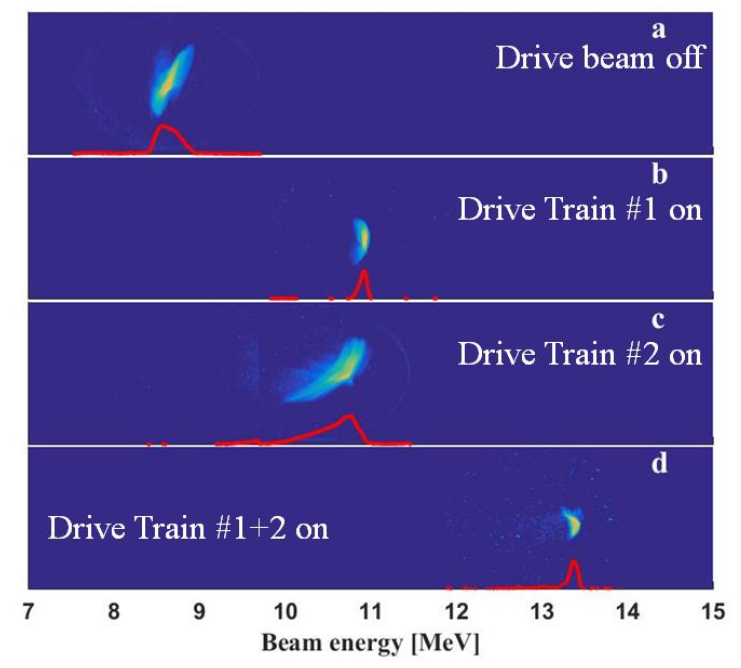
\includegraphics[width=0.75\textwidth]{images/old_tba}
	\label{fig:old-tba}
	\caption{Measurements of the energy during simplified staging experiments, 
		figure courtesy of G. Ha at AWA.
		Drive Train 1 refers to the stage one, and Drive Train 2 to stage 2. 
		Energy gain was observed in each stage independently.
		A larger energy gain was observed when both stages supplied RF to the witness beam line.}
\end{figure}
The biggest source of error is expected to be the transmission loss. 
%%%%%%%%%%%%%%%%%%%%%%%%%%%%%%%%%%%%%%%%%%%%%%%%%%%%%%%%%%%%%%%%%%%%%%%%%%%%%%%%%%%%%%%%%%%%




\Section{Modifications to Reach Fully Staged TBA} \label{sec:requirements}

In order to design and test fully staged TBA, a mechanism to route the drive beam into two independent beam lines had to be developed, along with an optics design for the new beam line. A kicker and a septum magnet will be used to route the beam. 
The kicker will provide a short Transverse Electric and Magnetic (TEM) field pulse
that will direct bunches into the bent beam line shown in Figure~\ref{fig:one}. 
This must be done with an electrostatic element as opposed to a magnet because 
the bunch spacing is too short to allow for the slow rise time of a magnetic field.
In addition the kick will be weak, so a septum magnet will be used to further
separate the two bunch trains. Simulations were used to determine hardware specifications such as the gap and plate dimensions of the kicker.

In addition to aiding the hardware design, simulations provide more realistic predictions of the beam dynamics in the machine, and allow optics design optimization.
Better simulations can help avoid problems such as the transmission loss in the second stage.
They can also reduce the amount of time spent on hand tuning the optics in the 
beam line during experiments.

%%%%%%%%%%%%%%%%%%%%%%%%%%%%%%%%%%%%%%%%%%%%%%%%%%%%%%%%%%%%%%%%%%%%%%%%%%%%%%%%%%%%%%%%%%%%
%%%%%%%%%%%%%%%%%%%%%%%%%%%%%%%%%%%%%%%%%%%%%%%%%%%%%%%%%%%%%%%%%%%%%%%%%%%%%%%%%%%%%%%%%%%%




\Section{Thesis Outline}

The rest of the thesis details work done at AWA Facility.
Chapter 2 covers experimental measurements and preparations for TBA.
The ultraviolet laser pulse train generation was modified, 
which improves the efficiency of RF power generation in the wakefield structures.
Measurements of the RF power in the gun and linac cavities are discussed.  
The beam diagnostics (energy, beam size, and bunch length measurements) are also described, including a description of beam size analysis and an image processing script written in Python. 
In Chapter 3 the simulation code, \verb|OPAL|~\cite{opal}, and the model used for the new beam line design are covered in detail.
Benchmarking of \verb|OPAL|, determination of optimization parameters, and comparison of optimization methods is described.  The \verb|OPAL| simulation was used to optimize the new drive beam line for TBA for a \SI{40}{nC} beam. 
In Chapter 4, the design of a stripline kicker needed to route beam into the new beam line is presented.
The achievable kicker angle and mechanical constraints at the AWA 
were used to lay out the fully staged TBA beam line. 
Simulations of the new beam line were done to ensure transmission at
the wakefield structure downstream. Optimization of the optics was done using 
a genetic algorithm and confirm that the configuration can transmit a \SI{40}{nC} beam, while maintaining a short bunch length needed for good power generation.



